\documentclass[english]{article}
\usepackage{amsmath}
\usepackage{amsfonts}
\usepackage{amssymb}
\usepackage{amsthm}
\newtheorem*{theorem}{Theorem}
\newtheorem*{lemma}{Lemma}
\newtheorem*{prop}{Proposition}
\newtheorem*{corr}{Corrolary}
\theoremstyle{definition}
\newtheorem*{defi}{Definition}
\newtheorem*{exa}{Example}
\theoremstyle{remark}
\newtheorem*{comm}{Comment}
\usepackage[english,ngerman]{babel}
\usepackage[latin1]{inputenc}
\newcommand{\f}[2]{\frac{#1}{#2}}							%short form: \frac
\newcommand{\Cases}[1]{\begin{cases}#1\end{cases}}			%short form: \begin{cases}...
\newcommand{\Enum}[2]{\begin{enumerate}[#1]#2\end{enumerate}}	%short form: \begin{enumerate}...
\usepackage[T1]{fontenc}
\usepackage{graphicx}
\usepackage{graphics}
\usepackage{float}

%% create an index 
\usepackage{makeidx}
\makeindex 
\newcommand{\M}{\mathcal{M}}
\newcommand{\N}{\mathcal{N}}
\newcommand{\E}{\mathcal{E}}
\newcommand{\p}{\partial}
\newcommand{\NN}{\mathbb{N}}			%creates symbol for natural numbers
\newcommand{\ZZ}{\mathbb{Z}}			%creates symbol for integral numbers
\newcommand{\II}{\mathbb{I}}				%creates symbol for irrational numbers
\newcommand{\PP}{\mathbb{P}}			%creates symbol for rational numbers
\newcommand{\QQ}{\mathbb{Q}}			%creates symbol for rational numbers
\newcommand{\RR}{\mathbb{R}}			%creates symbol for real numbers
\newcommand{\HH}{\mathbb{H}}			%creates symbol for quaternions
\newcommand{\RRn}{\RR^n}					%creates symbol for n-dim. real space
\newcommand{\CC}{\mathbb{C}}			%creates symbol for complex numbers
\newcommand{\CCn}{\mathbb{C}^n}		%creates symbol for complex numbers
\newcommand{\KK}{\mathbb{K}}			%creates symbol for a field
\newcommand{\euclid}{ \tx{euclid }}
\newcommand{\one}{\mathbb{1}}			%creates symbol for unity
\newcommand{\A}{\mathcal{A}}
\newcommand{\B}{\mathcal{B}}
\renewcommand{\L}{\mathcal{L}}
\renewcommand{\P}{\mathcal{P}}
\newcommand{\F}{\mathcal{F}}
\newcommand{\Q}{\mathcal{Q}}
\newcommand{\D}{\mathcal{D}}
\newcommand{\sig}{\sigma}
\newcommand{\case}{\begin{array}[h]{r}}
  \newcommand{\caseend}{\end{array}}
\renewcommand{\Im}{\tx{Im }}
\renewcommand{\Re}{\tx{Re }}
\newcommand{\minusone}{^{-1}}

\newcommand{\lam}{\lambda}			%creates symbol for \lambda
\newcommand{\Lam}{\Lambda}\newcommand{\GG}{\Gamma}
% creates symbol for \Lambda
\renewcommand{\aa}{\alpha}		%creates symbol for \alpha
\newcommand{\gam}{\gamma}			%creates symbol for \gamma
\newcommand{\bb}{\beta}					%creates symbol for \beta
\newcommand{\dd}{\delta}				%creates symbol for \delta
\newcommand{\ee}{\varepsilon}		%creates symbol for \varepsilon
\newcommand{\vphi}{\varphi}			%creates symbol for \varphi
\newcommand{\id}{\tx{id}}			%creates symbol for id
\newcommand{\y}{\left\langle }
  \newcommand{\yy}{\right\rangle }
\newcommand{\OO}{\Omega}
\newcommand{\ww}{\omega}
\newcommand{\DD}{\Delta}
\newcommand{\GL}{\tx{ GL }}
\newcommand{\cinf}{\tx{C}^\infty}
\newcommand{\drw}{\Rightarrow}			%creates symbol for \Rightarrow	| with reference
\newcommand{\dlw}{\Leftarrow}			%creates symbol for \Leftarrow		| to the symbol
\newcommand{\ot}{\leftarrow}
% creates symbol for \Leftarrow		| to the symbol
% creates symbol for \leftarrow		| \to looking like  -\yy 
\newcommand{\toto}{\longrightarrow}	%creates symbol for \rightsquigarrow:  ~\yy 
\newcommand{\gdw}{\Leftrightarrow}	%creates symbol for \Longleftrightarrow
\newcommand{\fa}{\ \forall}				%creates 'Space'+\forall
\newcommand{\ex}{\ \exists}				%creates 'Space'+\exists
\newcommand{\nex}{\ \nexists}			%creates 'Space'+\nexists
\newcommand{\cd}{\cdot}						%creates a short form for \cdot
\newcommand{\bs}{\backslash}			%creates a short form for \backslash
\newcommand{\bracks}[1]{\left\{#1\right\}}		%creates a brackets like {...} round the expression #1
\newcommand{\limes}[1]{\lim\limits_{#1}}%creates a \lim object and \limits beneath
\newcommand{\tri}{\nabla}
\newcommand{\End}{\tx{ End }}
\newcommand{\grad}{\tx{ grad }}
\newcommand{\supp}{\tx{ supp }}
\newcommand{\curv}{\tx{ curv }}
\newcommand{\Img}{\tx{ Img }}
\newcommand{\const}{\tx{ const }}	
\newcommand{\Span}{\tx{ span }}
\newcommand{\ric}{\tx{ Ric }}
\newcommand{\lightning}{ }
\newcommand{\rank}{\tx{ rank }}
\newcommand{\sign}{\tx{ sign }}
\newcommand{\Hom}{\tx{ Hom }}
\newcommand{\vol}{\tx{ Vol }}
\newcommand{\SU}{\tx{ SU }}
\newcommand{\SO}{\tx{ SO }}

\renewcommand{\div}{\tx{ div }}
\newcommand{\under}[2]{\underbrace{#1}{\text{#2}}}	%creates a \underbrace object defining #2 as a text
\newcommand{\stack}[2]{\stackrel{#1}{#2}}		%creates a \stackrel object defining #1 as a text
\newcommand{\tx}[1]{\text{#1}}
\newcommand{\sk}[1]{\y #1 \yy }					%creates a \text object
\newcommand{\ortho}{\bot}
\newcommand{\tbf}[1]{\textbf{#1}}
\newcommand{\tr}[1]{\tx{ tr }({#1})}

\begin{document}
\begin{titlepage}
  \begin{center}
    \ \\
    \vspace{03mm}
    {\huge Finite Element Methods\\}
    \vspace{12mm}
    {\Large by Dirk Klindworth}\\
    www.tu-berlin.de/?fem-lecture
    \vspace{12mm}\\
    {\Large  {SS 14\\ }}
    \vspace{15mm}
    {\Large written by Juri Schmelzer  \\
      graphics by Fred Brockstedt}
  \end{center}
\end{titlepage}
\newpage
\tableofcontents
\newpage
\section{Theoretically Background}
\begin{defi} a \index{differential equation}differential equation is an equation satisfied by a function $u$, which involves besides $u$ its derivatives
  \begin{enumerate}
  \item $u$ depends on only one variable (ordinary differential equations)
  \item $u$ depends on more than one variable ($\p_i u:= \f{\p u (z)}{\p z_i}$ partial differential equations (PDE))
  \end{enumerate}
\end{defi}
\subsection{Classification of PDE}
elliptic, hyperbolic, parabolic

\begin{enumerate}
\item elliptic \index{elliptic}: an incident at $z$ influences all points in the neighborhoods.
\item parabolic \index{parabolic}: there is one direction from $z$ where the influence is only for larger values
\item there are areas of influence
\end{enumerate}
\begin{defi} The principle part of the second order PDE \index{PDE}
  $$-\sum_{i,j=1}^n \p_i a_{i,j}(z)\p_j u(z) + \sum_{i=1}^n b(z)\p_i u(z) + c(z) u(z) = f(z)$$
  is $$\sum_{i,j=1}^n \p_i a_{i,j}(z) \p_j u_j(z)$$
\end{defi}
\begin{defi}
  \begin{enumerate}
  \item the PDE is elliptic \index{elliptic} at z if the eigenvalues of A are all non-zero and of the same sign
  \item parabolic \index{parabolic} if one eigenvalue is 0 and the rest all positive or all negative
  \item hyperbolic \index{hyperbolic} if n-1 eigenvalues have the same sign and on has the other sign
  \end{enumerate}
\end{defi}

\begin{exa} Stationary heat equation\\
  In absence of work the conservation of energy correspondents to the coversation of temperature
  $$f{\p u}{\p t}(x,t) + \tri j (x,t)= f(x,t)$$
  where
  \begin{enumerate}
  \item u is the temperature with unit [u]=1K
  \item j is the heat flux with unit [j]=$1\f{W}{m^2}$
  \item f is a heat source with unit [f]=$1\f{W}{m^3}$
  \end{enumerate}
  As constitutive equation (material property) we have Fouriers law 
  $$j(x,t)=-A(x)\tri u(x,t)$$
  We call the material 
  \begin{enumerate}
  \item homogeneous \index{homogeneous} if $A(x)=A$, inhomogenous otherwise
  \item isotropic \index{isotropic} if $A(x)= \aa(z)1,$ anisotropic otherwise
  \end{enumerate}
\end{exa}
For a unique solution u of constitutive equation we need initial conditions
$$u(x,0)= u_0 (x)$$
and boundary conditions \index{boundary condition} on boundary $\p \OO$ of $\OO$
\begin{enumerate}
\item $u(x,t)= g(x,t)$ for $x \in \p \OO, t>0$ (Dirichlet b.c.)
\item $j(x,t) n(x) = h(x,t)$ for $x \in \p\OO, t>0$ (Neumann b.c.)
\item $j(x,t) n(x) + \bb(x) u(x,t) = h(x,t)$ (Robin b.c.)
\end{enumerate}

\begin{figure}[H]
  \begin{center}
    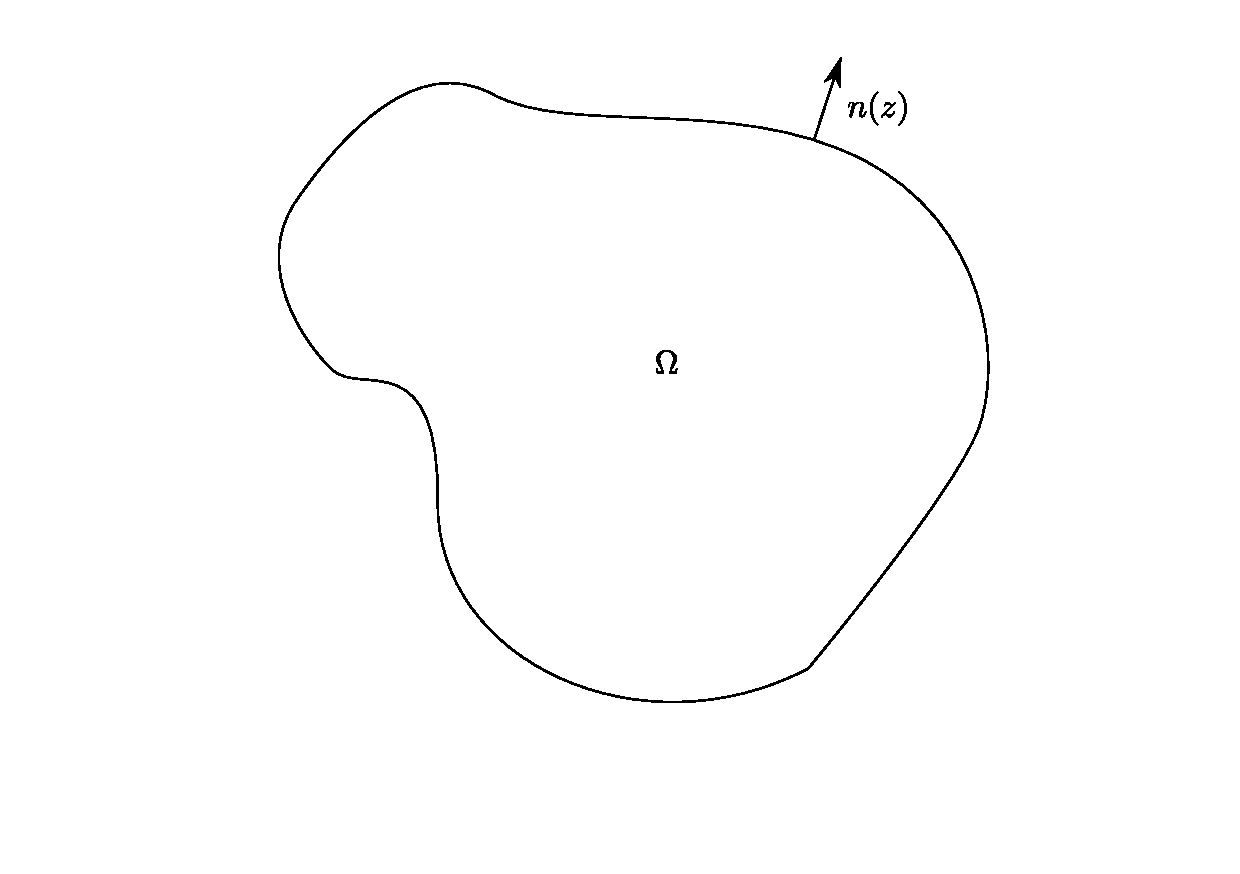
\includegraphics[width=\textwidth]{figs/OmegaDomain.pdf}
  \end{center}
  \caption{Illustration of a $\Omega$-domain for Neumann b.c.}
  \label{omega-domain-figure}
\end{figure}

Static emit of constitute equatation.\\
we suppose that the temperature does not change in time i.e. $\f{\p u}{\p t}=0$
$$\drw \tri j(x) = f,\ j(x)=-A \tri u \drw -\tri A(x)\tri u(x) = f(x) + b.c.$$


other examples\\
The same system arises in 
\begin{enumerate}
\item electro static, where u is the electric potential, j is the displacement field (usually denoted by D), f is the charge density (usually denoted by $\rho$)
\item stationary electric currents, where u is the electric potential and j is the electric current, f=0
\end{enumerate}
Well posedness\\
\begin{defi} A problem is said to be well posed if 
  \begin{enumerate}
  \item it has a unique solution $u$, and
  \item the solution depends continuously on the given data f i.e. $||u||\leq C ||f||$
  \end{enumerate}
\end{defi}
Recall transient/stationary heat equation
$$\underbrace{\f{\p u}{\p t}}_{=0 \tx{in case of stationary h.eq}}+ \nabla j = f$$
$$j= -A(x)\nabla u$$
with b.c's
\begin{enumerate}
\item $u(x) = g(x)$ (Dirichlet)
\item $j(x) n(x) = h(x) $ (Neumann)
\item $j(x)n(x) + \bb (x) u(x) = h(x) $ (Robin)
\end{enumerate}
\subsection{Elliptic boundary value problem}
\begin{comm}abstract notation:\\
  \begin{align*}
    -\nabla a \nabla u + c u &= f& \tx{in } \OO\subset\RR^d,d=1,2,3\\
    u&=g & \tx{on }\GG_D \subset \p \OO\\
    a\nabla u n&=h &\tx{on } \GG_N \subset \p \OO \\
    a \nabla u n + \bb u &= h & \tx{on }\GG_{R}\subset \p \OO
  \end{align*}
  $Re(c)\geq 0$, $0<\aa_0\leq Re(a) \leq a \leq \infty$\end{comm}
\begin{defi}classical Solution:\\
  If $u \in C^2(\OO)\cap C(\bar\OO)$ satisfies the PDE as well as the b.c's in a pointous sense, then u is called classical \index{classical solution} solution of the BVP
\end{defi}
\begin{comm}
  \begin{enumerate}
  \item existence of classical solution is a requirement of some numerical scheme, e.g. the finite difference method (FDM)
  \item this requirement will be weakened when introducing the variational formulation.
  \end{enumerate}
\end{comm}
\begin{corr}
  Small perturbation in the data of a linear, well posed problem lead to small perturbation of the solution
\end{corr}
Proof: $\tilde f = f + \delta f , \delta f <<1$, then $a \tilde u$ solves the problem with data $\tilde f$ and $\delta u = \tilde u - u$ solves the problem with the data of $\drw ||\delta u || \leq C||\delta f||$

\begin{exa} how to proof well-posed (Serial 1 1.b)\\
  find $u(x,1) $ with initial data $sin(n\pi x) ,\ n \in \NN$
  \begin{align*}
    \tilde u (x,0) &= sin(\tilde n \pi x)& \tx{subst. } s=\tilde n \pi x\\
    ||\tilde u (x,0)||^2_{L^2(-1,1)} &= \int^1_{-1}sin^2(\tilde n \pi x) dx &=... = 1\\
    \tilde u (x,t=1) &= e^{-\tilde n^2\pi^2}sin(\tilde n \pi x)\\
    ||\tilde u (x,1)||_{L^2}&= \sqrt{e^{-\tilde n ^2 \pi^2}}||\tilde u(x,0)||_{L^2} 
    &\leq \underbrace{C}_{=1} ||\tilde u (x,0)||_{L^2} &\quad
  \end{align*}
\end{exa}
\subsection{Numerical solutions of elliptic BVP}
\begin{comm}
  Closed form solution versus numerical solution
  \begin{enumerate}
  \item only most elementary PDE have closed form solutions
  \item but even if they exist, there value can be questioned
  \end{enumerate}
\end{comm}
\begin{exa}
  Consider Poisson Problem equation\\
  \begin{align*}
    -\tri u &= 2 & \tx{in }\OO\in (-1,1)^2\\
    u&=0 & \tx{on }\p\OO
  \end{align*}
  The closed form solution looks like this:

  $$u(x,y) = 1 - y^2 -\f{32}{\pi^3} \sum_{n=1}^\infty \f{(-1)^k cosh(\f{2k+1}{2}\pi x) cos(\f{2k+1}{2}\pi y)}{(2k+1)^3cosh(\f{2k+1}{2}\pi)}$$
  Problems:
  \begin{enumerate}
  \item infinite sum need to be truncated: very often the amount of terms of the sum is prohibitively large to sufficient accuracy
  \item for large k $$\f{cosh(\f{2k+1}{2}\pi x)}{cosh(\f{2k+1}{2}\pi)}$$
    the numerical calculations is far from trivial.
  \item A modification of the b.c's may result in a totally different schemes.
    
  \end{enumerate}
\end{exa}
\subsubsection{Finite Difference Method (FDM)}
If a classical solution of the BVP exists (which implies that $u\in C^2(\OO)$), we can replace the derivatives by different quotients.\\

Let d=1 and $\OO\subset \RR$ be an interval, h>0, Then, if $u \in C^{n+1}(\OO)$ then we can employ the  Taylor theorem, which gives:
$$u(x\pm h) = u(x)\pm hu'(x) + \f{h^2}{2}u''(x) + ...+\f{\pm h^n}{n!}u^{(n)}(x)+ R_n(u,x,h)$$
with the remainder 
$$R_n(u,x,h)=\f{1}{n!}\int^{x\pm h}_x (x-t)^n u ^{n+1}(t)dt= \f{\pm h^{n+1}}{(n+1)!} u^{(n+1)(\eta)}$$
for some $\eta \in [x,x\pm h]$\\
\begin{enumerate}
\item $\drw$ first order forward difference quotient\\
  $$\f{u(x+h) -u(x)}{h}= u'(x) + \O(h)$$
\item $\drw$ first order backward difference quotient\\
  $$\f{u(x) -u(x-h)}{h}= u'(x) + \O(h)$$
\item $\drw$ second order centered difference quotient\\
  $$\f{u(x+h) -u(x-h)}{2h}= u'(x) + \O(h^2)$$
\item $\drw$ standard d.q.\\
  $$\f{u(x+h) -2u(x) +u(x-h)}{h^2}= u''(x) + \O(h^2)$$
\end{enumerate}
advantages of FDM
\begin{enumerate}
\item easy to implement
\item system matrix is sparse
\item convergent solution in $l_\infty$-norm
\end{enumerate}
disadvantages of FDM
\begin{enumerate}
\item required of classical solution
\item a(x) needs to be continuously diff.
\item limitation to simple domains
\item point-wise approximation
\end{enumerate}
\subsubsection{Finite Element Method}
\begin{enumerate}
\item weaker requirement on the regularity of the solution/ material function
\item possibility for more complicated domains
\end{enumerate}
\begin{comm}
  Key ingredients
  \begin{enumerate}
  \item transformation of BVP from strong formation to a so-called variational \index{variational} (weak) formation
  \item Discretization of the computational domain $\drw$ irregular meshes instead of grid

    \begin{figure}[H]
      \begin{center}
        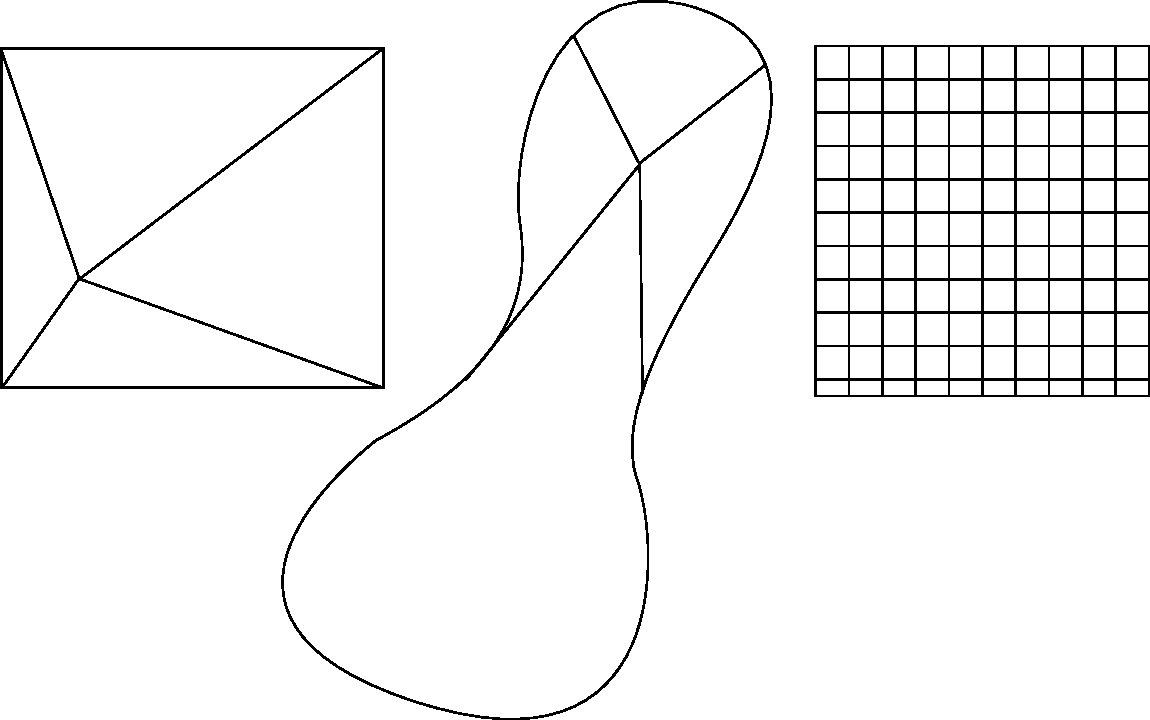
\includegraphics[width=\textwidth]{figs/differentGrids.pdf}
      \end{center}
      \caption{Different types of grids}
      \label{different-grids-figure}
    \end{figure}

    \begin{itemize}
    \item based on mesh we define basis functions of discrete sup-space of the space where we look for the weak solution
    \item basic solutions have a local support
    \end{itemize}
  \end{enumerate}
\end{comm}

\section{Variational Formation}
\subsection{computational domain}
\begin{defi}
  \begin{itemize}
  \item domain $\OO$: bounded, connected, open subset of $\RR^d$, d=1,2,3
  \item boundary $\p\OO:=\bar\OO \backslash \OO$ at least $C^0-$continuous and closed.
  \end{itemize}
  Furthermore, the domain needs to be a Lipschitz-domain
  \begin{itemize}
  \item boundary is of finite length (excluding fractal boundaries)
  \item boundary slightly smoother than continuous (excluding slit/cusp domains)
  \end{itemize}
\end{defi}

\begin{figure}[H]
  \begin{center}
    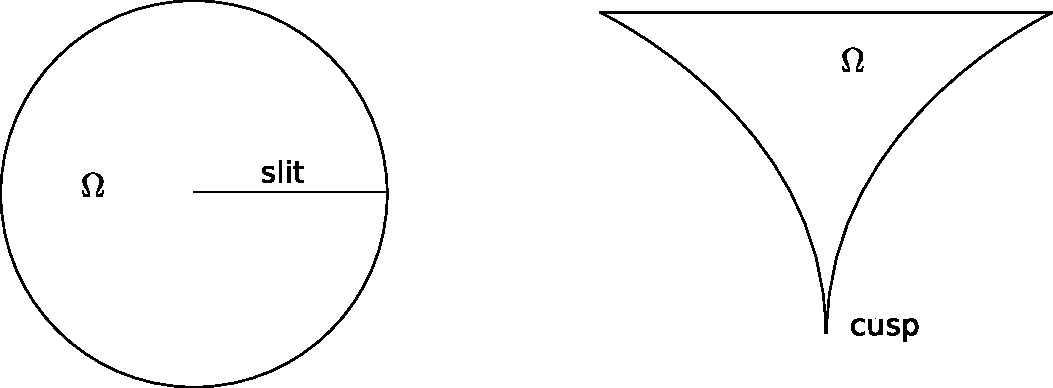
\includegraphics[width=\textwidth]{figs/notLipschitzDomain.pdf}
  \end{center}
  \caption{Domains that are not Lipschitz}
  \label{not-lipschitz-figure}
\end{figure}

\begin{comm}
  In practice only domains can be described by CAD software are relevant. This set of domains is usually equivalent to the following set of domains\end{comm}

\begin{defi}
  Let d=2. A connected domain $\OO$ is called  \index{curvilinear} \emph{curvilinear Lipschitz-polygon} if 
  \begin{itemize}
  \item $\OO$ is Lipschitz
  \item there is a finite number of open subsets $\GG_K\subset \p\OO, k=1,...,p\in \NN$, such that 
    $$\p\OO=\bar\GG_1\cup....\cup \bar\GG_p,\ \GG_k\cap \GG_l=\emptyset \ \forall k\neq l$$
    and for each $k\in\left\{1,...,p\right\}$ there exists a $C^1-$diffeomorphism (invertible mapping of smooth manifolds) $\Phi_k : [0,1]\to \GG_k$
  \end{itemize}
\end{defi}

\begin{figure}[H]
  \begin{center}
    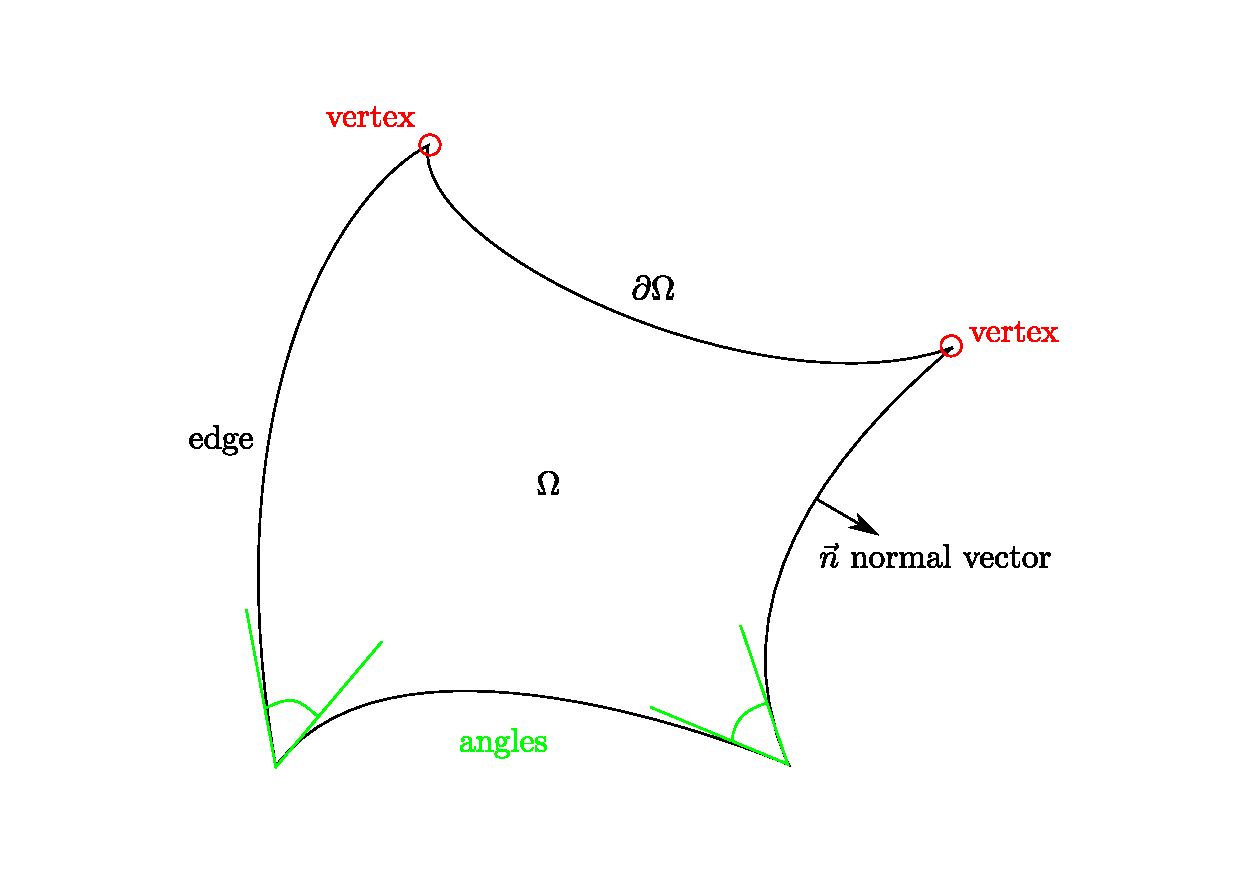
\includegraphics[width=\textwidth]{figs/curvilinear.pdf}
  \end{center}
  \caption{curvilinear domain}
  \label{curvilinear-domain-figure}
\end{figure}

\begin{defi}
  A subset $\OO\subset \RR^d$ is called \emph{computational  domain} \index{computational} if it is bounded and its boundary is $C^1-$continuous, or if it is 
  \begin{itemize}
  \item bounded connected interval(d=1)
  \item a curvilinear Lipschitz-polygon(d=2)
  \item a curved Lipschitz-polyhedron(d=3)
  \end{itemize}
\end{defi}
\subsection{Linear differential operator}
\begin{defi}
  Let $\aa \in \NN_0 ^b$ be a multi-index and $|\aa| = \aa_1+...aa_d$. Then we call 
  \begin{itemize}
  \item $$\p^\aa:=\f{\p^{\aa_1}}{\p x_1^{\aa_1}}...\f{\p^{\aa_d}}{\p x_d^{\aa_d}}$$
    the \emph{partied deriviate of order} $|\aa|$\\
  \item the \emph{gradient} of a function f 
    $$\nabla f (x) = (\f{\p f}{\p x_1}(x),...,\f{\p f}{\p x_p}(x))^{(T)}$$
  \item \emph{divergence} of a vector field $ f=(f_1,...,f_d)^{(T)}$
    $$\nabla \cdot f(x) = \sum_{i=1}^d \f{\p f_i}{\p x_i}(x)$$
  \item \emph{Laplacian}
    $$\Delta :=\tri \cdot \tri$$
  \end{itemize}
\end{defi}
\subsection{Integration by parts}
\begin{theorem} Gau\ss{}-Theorem\\
  If $f \in(C^1(\OO))^d\cap (C^0(\bar\OO))^d$ then 
  $$\int_\OO \tri \cdot f d\ x = \int_\GG f \cdot n d\ s$$
  By the product rule $\tri \cdot (u f )= u \tri \cdot f + \tri u \cdot f$ we deduce the Green's formula
  $$\int_\OO f \cdot \tri u + \tri \cdot f u d\ x = \int_\GG f \cdot n u d\ s$$
  for all $f \in(C^1(\OO))^d\cap (C^0(\bar\OO))^d$ and $u \in(C^1(\OO))^d\cap (C^0(\bar\OO))^d$
\end{theorem}
\begin{exa}
  \begin{itemize}
  \item $f=f e_k$ where $e_k$ is the k-th unit vector
    $$\drw \int_\OO f \f{\p u}{\p c^k}+ \f{\p f}{\p x_k} u d\ x = \int_\GG f u(n)_k d\ s$$
  \item $f = \nabla v, v \in C^2(\OO)\cap C^1(\bar\OO)$
    $$\drw \int_\OO \nabla u \cdot \nabla v + \Delta v u d\ x = \int_\GG \nabla v n d\ s$$
    
  \end{itemize}
\end{exa}
\subsection{Distributional derivations}
\begin{defi} Test function space\\
  For a non-empty open set $\OO \subset \RR^d$ we denote 
  $$\cinf_0 (\OO) := \left\{v \in \cinf(\OO) : supp\ v := \left\{x \in \OO: v(x)\neq 0 \right\} \subset \OO\right\}$$
  the space of test functions
\end{defi}
\begin{lemma}
  Two integral functions f and g defined in the bounded set $\OO$ are almost everywhere equal 
  $$\gdw \int_\OO f v d\ x = \int g v d\ x$$
  for all test functions $v \in \cinf_0(\OO	)$
\end{lemma}
\begin{defi}
  Let $u \in L^2(\OO)$ and $\aa \in \NN^d _0$. A function $w \in L^2(\OO)$ is called \emph{weak derivative} \index{weak derivative} or \emph{distributional derivative} \index{distributional derivative} $\p^\aa u$ (of order $|\aa|$) of u, if 
  $$\int w v d\ x = (-1)^{|\aa|} \int _\OO u \p^\aa v d\ x$$
  for all $v \in \cinf_0(\OO)$

\end{defi}

\begin{itemize}
\item weak gradient $w \in (L^2(\OO))^d$ of $u \in L^2(\OO)$
  $$\int w\cdot v d\ x = -\int u \nabla \cdot v d\ x$$
  for all $v \in (\cinf_0 (\OO))^d$
\item weak divergence $w\in L^2(\OO)$ of $u \in (L^2(\OO))^d$
  $$\int w\cdot v d\ x = -\int u \cdot\nabla  v d\ x$$
  for all $v \in \cinf_0(\OO)$
\end{itemize}
\begin{theorem}
  If $u \in C^m(\bar\OO)$ then all weak derivatives of order $\leq 0$ agree in $L^2(\OO)$ with the corresponding classical derivative.
\end{theorem}
\begin{comm}Extension of integration by parts\\

  For Lipschitz domains the Gau\ss{}-theorem (and hence also (7G7)) can be extended to integrable functions with weak derivative
\end{comm}
\begin{comm} Weak derivatives in sub domains\\
  The weak derivative in $\OO$ and in a sub domain $\OO_1 \subset \OO$ coincide in $\OO_1$ since the space of test functions satisfy $\cinf_0(\OO) \subset \cinf_0(\OO_1)$
\end{comm}
\begin{comm} Continuity over interfaces of sub domains\\
  For the partition $\bar\OO = \bar\OO_1 \cup \bar\OO_2, \OO_1\cap\OO_2=\emptyset,$ where both sub domains are supposed to have a Lipschitz boundary, a function u, which has a weak gradient in $\OO_1$ and $\OO_2$has a weak gradient in $\OO$ if and only if $[u]_2 = 0$ $$\sum:= \p \OO_1 \cap\p \OO_2$$
\end{comm}
\begin{defi} extra remarks to computational domain\\
  An open, connected set $\OO \subset \RR^d $ is called \emph{Lipschitz-domain} \index{Lipschitz-domain}, if its boundary $\p\OO:=\bar\OO\backslash \OO$ is \emph{Lipschitz boundary} which is equivalent to 
  \begin{itemize}
  \item $\exists$ finite covering of $\p\OO$ of open subsets of $\RR^d$, and 
  \item $\p \OO$ i locally (for each open rectangle) the graph of a Lipschitz continuous function
  \end{itemize}
\end{defi}
\begin{defi}
  curvi linear Lipschitz polygon\\
  d=2 \ A Lipschitz domain $\OO\subset \RR^d$ is called a \index{c.L.p.} c.L.p. if $\exists $ finite number of open subsets $\GG_k \subset \p \OO$, $k=1,...,P, P\in \NN$ s.t. $\forall k \exists C^1$-diffeomorphism $\Phi_k : [0,1] \to \GG_k$

\end{defi}
\subsection{Variational formulations of elliptic BVPs}
\begin{comm}
  Recall BVP 1.4
  \begin{align}
    -\tri \cdot a \tri \cdot u + su &= f& in\ \OO\\
    u&=g &on\ \GG_D
    a \tri u \cdot n &= h& on\ \GG_N\\
    a\tri u \cdot n + \bb u &= h& on\ \GG_R
  \end{align}
  and Eq(2.4), weak divergence $w \in L^2(\OO)$ of $u \in (L^2(\OO))^d$
  $$\int_\OO w v d\ x = - \int_\OO u \cdot \tri v d\ x \ \forall v \in \cinf_0(\OO)$$
\end{comm}
\subsubsection{Pure Dirichlet b.c.'s}
\begin{comm}
  $$\int_\OO (-\tri \cdot a \tri u + cu)v d\ x = \int_\OO fv d\ x \ \forall v\in\cinf_0(\OO)$$
  $$\overbrace{\drw}^{2.4} \int_\OO a \tri u \cdot \tri v + cuv d\ x = \int_\OO fv d\ x \ \forall v\in\cinf_0(\OO)$$
  $u=g$ becomes an \emph{essential b.c.}, i.e. it is incorporated into the space of test and trial functions
\end{comm}
\subsubsection{Pure Neumann b.c.'s}
$$\int_\OO (-\tri \cdot a \tri u + c u) v d\ x = \int_\OO f v d\ x \ \forall v \in \cinf(\bar\OO)$$
FGF
$$\int_\OO f \cdot \tri u + \tri \cdot f u d\ x = \int_\GG f\cdot n u d\ S(x)$$
$$f= a \tri u \drw \int_\OO a\tri u \cdot \tri v d\ x - \int_\GG a \tri u \cdot n v d\ S(x)=-\int_\OO \tri \cdot a \tri u v d\ x$$
$$\drw \int_\OO a \tri u \cdot \tri v + c u v d\ x - \int_\GG \underbrace{a\tri u \cdot n}_{=h} v d\ S(x) = \int_\OO f v d\ x \ \forall v\in\cinf(\bar\OO)$$
Boundary condition which are present in the variational formulation are called \index{natural boundary condition} natural b.c.
\subsubsection{Robin b.c.'s}
$$\int_{\OO}a \tri u \cdot \tri v + c u v d\ x - \int_\GG \underbrace{a \tri u}_{h-\bb u} \cdot n v d\ S(x) = \int_\OO f v d\ x$$
$$\int_\OO a \tri u \cdot \tri v + c u v d\ x + \int_\GG \bb u v d\ S(x) = \int_\OO f v d\ x + \int_\GG g v d\ S(x) \forall v \in \cinf (\bar\OO)$$







? order of the next part?
\begin{exa} 
  $\OO= (0,1).$ Give an example of a function $u \in C^1(\OO)$ that does not posses a weak gradient bounded in $L^2(\OO)$\\
  Recall Thm 2.7.\\
  If $u \in C^m(\bar\OO)$, then all weak derivatives of order $\leq m$ agree in $L^2(\OO)$ with the classical derivative\\
  For example:
  \begin{align*}
    f(x) &= ln\ x\\
    f'(x)&=\f{1}{x}\\
    ||f'||_{L^2}^2&= \int_0 ^1 (f')^2 d\ x\\
    -f(x) = \sqrt{x}
    \vdots
  \end{align*}
\end{exa}
%% missing part added by Fred
\subsection{Linear and bilinear forms}
Let $V,W$ be real/complex vector spaces
\begin{itemize}
\item \index{Linear operator}\emph{Linear operator} is a mapping
  \begin{eqnarray*}
    T:V & \to & W\\
    T\left(\lambda v+\mu w\right) & = & \lambda T\left(v\right)+\mu T\left(w\right)
  \end{eqnarray*}
  $\forall v,w\in V$ and $\lambda,\mu\in\mathbb{R}$ or $\mathbb{C}$.
\item \index{Linear form}\emph{Linear form} is a linear operator $l:V\to\mathbb{R}$
  or $\mathbb{C}$.
\item \index{Bilinear form}\emph{Bilinear form} is a mapping
  \[
  b:V\times V\to\mathbb{R}\mbox{ or }\mathbb{C}
  \]
  where $v\mapsto b\left(v,w\right)$ $\forall w\in V$ and $w\mapsto b\left(v,w\right)\forall v\in V$
  are linear forms
  \[
  \underset{=b\left(u,v\right)}{\underbrace{\int_{\Omega}a\nabla u\cdot\nabla v+cuv\ dx}}=\underset{=l\left(x\right)}{\underbrace{\int_{\Omega}fv\ dx}}
  \]

\item \index{Antilinear operator}\emph{Antilinear operator} is a mapping
  \begin{eqnarray*}
    T:V & \to & W\\
    T\left(\lambda v+\mu w\right) & = & \bar{\lambda}T\left(v\right)+\bar{\mu}T\left(w\right)
  \end{eqnarray*}
  $\forall v,w\in V$, $\forall\mu,\lambda\in\mathbb{C}$.
\item \index{Antilinear form}\emph{Antilinear form} is a antilinear operator
  $l:V\to\mathbb{C}$.
\item \index{sesquilinear form}\emph{sesquilinear form} is a mapping
  \begin{eqnarray*}
    b:V\times V & \to & \mathbb{C}
  \end{eqnarray*}
  such that $v\mapsto b\left(v,w\right)$ is a linear form $\forall w\in V$
  and $w\mapsto b\left(v,w\right)$ is a antilinear form
\end{itemize}

\paragraph{Properties of bi-/sesquilinear forms}
\begin{itemize}
\item symmetric $b\left(u,v\right)=b\left(v,u\right)$
\item positive definite $\left|b\left(v,v\right)\right|=0\iff v\neq0$
\item V-continuous (or V-bounded) $\left|b\left(u,v\right)\right|\le\underset{\mbox{continuity constant}}{\underbrace{\left|\left|b\right|\right|}\left|\left|u\right|\right|_{V}\left|\left|v\right|\right|_{V}}$
  $\forall u,v\in V$
\item V-elliptive (also coercive) $\left|b\left(v,v\right)\right|\ge\underset{\mbox{ellipticity constant}}{\underbrace{\gamma}\left|\left|v\right|\right|_{V}^{2}}$
  $\forall v\in V$
\end{itemize}
A symmetric positive definite bi-/sesquilinear form is an \emph{inner
  product\index{inner product}} that induces a norm
\[
\left|\left|v\right|\right|_{b}:=\left|b\left(v,v\right)\right|
\]
In the context of elliptic PDEs, if the bi-/sesquilinear form $b$
in (LVP) is symmetric, positive definite, it is called \emph{energy
  norm}\index{energy norm} $\left|\left|\cdot\right|\right|_{e}$.

%% missing part end

\subsection{Sobolev spaces}
\begin{defi}
  A normed vector space V is complete, if every Cauchy sequence $\left\{ v_k \right\}_k \subset V$ has a limit in V. A normed, complete vector space is called \index{Banach space}Banach space\end{defi}
\begin{defi}
  A Hilbert space is a Banachspace whose norm is induced by a inner product.\end{defi}
Recall variational formulation of BVP with pase, homogeneous Neumann b.c.
$$\int_\OO a \tri u \cdot \tri v + cuv d\ x = \int_\OO fv d\ x$$
for all test functions v$\in \cinf _0(\OO)$\\
\emph{Ideal space} of u and v in 2.9. is a Hilbert space whose inner product coincides with the bilinear form, i.e. it is equipped with the energy norm
$$||v||_e ^2 = \int |a||\tri v |^2 +|c||v|^2 d\ x $$
and the space is defined as 
$$ H:= \left\{v : \OO \to \RR | \tx{weak gradient }\tri v \tx{ exists and } ||v||_e <\infty \right\}$$
The same applies also to the test function, that are now more functions than in $\cinf_0$(equatation due to Meyser-Serrin Theorem, see Thm.2.15)
\begin{defi}
  The Sobolev space $H^1(\OO)$ is the space of all square integrable function's with square integrable weak gradients
  $$H^1(\OO) := \left\{v\in L^2(\OO) : \tx{weak gradient }\tri v \tx{ exists and } ||\tri v||_{L^2} <\infty \right\}$$
  with norm $$||v||^2 _{H^1(\OO)} = ||v||^2 _{L^2(\OO)} + D^2 ||\tri v||_{L^2(\OO)}$$
  where $D= diam (\OO)$ to meet unit ....


  The $H^1$-norm and the energy norm are equivalent if the latter is base on a $H^1-$elliptic and $H^1-$continuous bilinear form, i.e. $\exists C_1,C_2>0$ such that:
  $$C_1 ||v||_e \leq ||v||_{H^1 }\leq C_2||v||_e \ \forall v \in H^1(\OO)$$
\end{defi}
\begin{defi} For $m \in \NN_0$ and $\OO\subset \RR^d$ we define the Sobolev of order m as ...
\end{defi}

\begin{theorem} 2.15. Meyser-Serrin theorem\\
  The space $C^\infty(\bar\OO)$is a dense subspace of $H^m(\OO)$ for all $m \in \NN_0$
\end{theorem}
\begin{defi}
  $H^1 _0 (\OO)$ is defined as the completion of $\cinf_0(\OO)$ with respect to the $H^1-$norm
\end{defi}
\begin{exa}
  Consider
  \begin{align*}
    -\tri \cdot a \tri u + cu & = f & \in \OO \\
    u                         & =0  & on\ \p\OO
  \end{align*}
  solution:
  \begin{align*}
    (a) & \int_\OO a \tri u \cdot \tri v + cuv d\ x & = \int_\OO fv d\ x + \int_{\p\OO} \tri u \cdot n v d\ s(x) & \forall v \in \cinf_0(\OO)                 \\
    (b) & ||v||_e ^2                                & := \int_\OO a \tri v \cdot \tri v + cvv d\ x                                                            \\
    & ||v||_e ^2                                & \geq 0                                                     & \forall v \in V=H_0 ^1 \drw a,c\geq \gg >0 \\
    (d) & \tx{Is }b \ H^1 _0-\tx{elliptic}?                                                                                                                   \\
    & \exists \gg>0:|b(v,v)|                    & \geq \gg_e||v||_{H^1}^2                                    & \forall v \in H_0 ^1(\OO)                  \\
    & |b(v,v)|                                  & \geq\gg\int_\OO (\tri v)^2 + v^2 d\ x                                                                   \\
  \end{align*}
\end{exa}
\subsection{Theory of variational formulations}
\subsubsection{Elliptics and the Lemma of Lax-Milgram}
\begin{defi} The dual V' of a normal vector space V is the normed vector space of continuous linear forms on V. The dual space is equipped with the operator norm 
  $$||f||_{V'} := sup\ _{v \in V\backslash \left\{0\right\}} \f{f(v)}{||v||_V}$$
\end{defi}
\begin{theorem}2.21 Lemma of Lax-Milgram\\
  Let V be a reflexive Banach space. Let bilinear form $b:V \times V \to \RR$ or sesquilinear form $b:V\times V \to \CC$ be V-elliptic. Then, the variational problem (LVP), i.e. $b(u,v) = l(v)$ has for any $f \in V'$ a unique solution $u \in V$ with 
  $$||u||_V \leq \f{1}{\gg_e}||f||_{V'}$$
\end{theorem}
\subsubsection{ The inf-sup conditions }
\begin{theorem}
  The following statements are equivalent
  \begin{enumerate}
  \item For all $f \in V'$ the linear variational Problem (LVP) has a unique solution $u \in U$ that satisfies 
    $$||u||_U \leq \f{1}{\gg}||f||_{V'}$$
    with $\gg>0$ independent of f\\
  \item The bilinear form b satisfies the \emph{inf-sup-conditions}
    $$\exists \gg >0: inf\ _{w \in U \backslash\left\{0\right\} } sup\ _{v \in V \backslash \left\{0\right\}} \f{|b(w,v)|}{||v||_v||w||_U} \geq \gg \ (IS1)$$
    $$\forall v \in V \backslash\left\{0\right\} : ... sup\ _{w \in U \backslash\left\{0\right\}} b(w,v)>0 \ (IS2)$$
  \end{enumerate}
\end{theorem}

\begin{exa}
  3.1.\\
  Solution:\\
  $$sup\ _{v \in V \backslash\left\{0\right\}} \f{|b(w,v)|}{||w||_U ||v||_V} \geq \f{|b(,w,w)|}{||w||^2}\geq \gg$$
\end{exa}
\begin{exa}3.2\\
  $b(u,v) = l(v) \forall v \in V$\\
  show that if IS1 is not than more than on solution exists, and if IS2 does may not exists a solution.\\
  (a)\\
  $U\neq U, \ b(u,v) =0$ \\
  with not IS1 follows : $$inf\ sup\ \f{|b(v,w)|}{||w||_U||v||_V} =0$$
  $u=w \drw b(u,v) = 0$
  (b)\\
  Suppose $\exists u \in U s.t.\ b(u,v) = l(v) \forall v \in V$ Now take the v which negates IS2.\\
  With perticular testfunctions we get $0= b(u,v') =l(v')\neq 0$ for $l(v) = \int_\OO v d\ x$
\end{exa}
\subsection{well-posedness of elliptic BVPs}
\subsubsection{BVP's with Dirichlet b.c.}
\begin{comm}
  \begin{align*} \\
    -\nabla \cdot a \nabla u + cu &=f & in\ \OO\\
    u &=g & in\ \p\OO\\
    \int_\OO a \nabla u \cdot \nabla v + cuv d\ x &= \int_\OO fv d\ x & \forall v \in V = ?
  \end{align*}
  $U = H^1 _g (\OO) := \left\{v \in H^1 (\OO) | v = g on\ \p\OO \right\}, V= H^1 _0(\OO)$\\
  Suppose u = g on $\GG_D \subset \p \OO$ then we write $$U= H^1 _{\GG_D,g}, V= H^1_{\GG_D, 0}$$
  $H^1 _g(\OO)$ is not a vector space if $g \neq 0$\\
  $u\in H^1 _g(\OO)  \drw \lam u \notin H^1 _g(\OO) if\ \lam \neq 1$\\
  We can equivlenlty write $$u = u_0 + u _g with\ u_g \in H^1_g(\OO) and\ u_0 \in H^1 _0 (\OO)$$
  $\drw$ find $u_0 \in H^1 _0 (\OO) s.t.\ $ 
  $$\int_\OO a \tri u_0 \cdot \tri v + c u_0v d\ x = \int_{\OO}f v d\ x - \int_\OO a \tri u_g \cdot \tri v + c u_g v d\ x$$
  for all $v \in H^1 _0(\OO)$\\
  For which function g can we find an extension $u_g \in H^1_g (\OO)$?\\
  \begin{itemize}
  \item Any restriction (trace) of a function $v\in H^1(\OO)$ to $\GG_D$ can be extendend to $u_g=v \in H^1(\OO)$.\\
  \item We can choose any function $u_g$ for which $u_g = g$ on $\GG_D$\\
  \item Let $\GG_D = \p\OO$ the trace span of $H^1(\OO)$ is $H^{\f{1}{2}}(\p\OO) \subset L^2(\p \OO)$
    $$||v||_{H^{\f{1}{2}}(\p\OO)} : = inf\ \left\{||w||_{H^1(\OO)} : w \in \cinf (\bar\OO) , w_{|\p\OO} = v\right\}$$
  \item For all functions $g \in H^{\f{1}{2}}(\p\OO)$ an extension exists.
  \item But also for all $g\in L^2 (\p \OO)$? NO! Think of discontinuing g.
  \end{itemize}
\end{comm}
For well posedness we have to prove 
$$|b(v,v)|\geq \gg ||v||^2 _{H^1(\OO)} \ \forall v \in H^1 _0 (\OO)$$
$$b(u,v) = \int_OO a \nabla u \cdot \nabla v + cuv d\ x$$
Recall that $s\geq a_0 >0, c\geq 0$\\
\begin{enumerate}
\item $c\geq c_0 >0$\\
  $$||v||^2_{H^1} = \int_\OO \nabla v \cdot \nabla v + vv d\ x$$
  $$b(v,v)\geq min\ \left\{a_0,c_0 \right\}\int_\OO \nabla v \cdot\nabla v + vv d\ x$$
\item c=0 with 2.24 \\
  $$b(v,v)\geq a_0\int_\OO \nabla v \cdot \nabla v d\ x \geq \f{a_0}{2}||\nabla v||^2_{L^2(\OO)} + \f{a_0}{2C_F}||u||^2_{L^2(\OO)}$$
  $$\geq \f{1}{2} min\ \left\{a_0, \f{a_0}{C_F}\right\} ||v||^2 _{H^1(\OO)}$$
\end{enumerate}
\begin{lemma}2.24 (Friedrichs inequality)\\
  Let $\OO$ be an open, bounded domain and $|\GG_D| >0$. Then for all $u \in H^1_{\GG_D,0}(\OO) $ there exists a constant $C_F(\OO,\GG_D)$ s.t. 
  $$||u||^2_{L^2(\OO)} \leq C_F diam\ (\OO)^2 ||\nabla u||^2 _{L^2(\OO)}$$
\end{lemma}
\newpage


missing lecture 8.5.2014



\newpage
\begin{comm}
  well-posedness of (DVP)
  \begin{itemize}
  \item for classical Galerki discretization with: $V_m\subset V$ well-posedness of DVP follows directly from V-elliticity of b.
  \item quasi optimality (Cea's Lemma)
  \item for grneral bi-/sesquilinear forms we need besudes IS1 and IS2 that the discrete inf-sup-condition is fullfilled\\
    $$\exists \gg_n >0 : inf\ _{w_n \in W_n\backslash \left\{0\right\}} sup\ _{v_n \in V_n\backslash \left\{0\right\}} \f{|b(w_n,v_n)|}{||w_n||_W||v_n||V} \geq \gg_n \ DIS$$
  \item one cannot conclude DIS from IS1 and IS2 since the supremum is taken over a much smaller set 
  \item $\gg_n\geq \gg_0>0:$ asymptotic quasi optimality estimate
    $$||u - u_n||_v \leq (1 + \f{||b||}{\gg_n})inf\ _{w_n \in W_n} ||u-w_n||_V$$
  \end{itemize}
  \subsection{ Algebraic setting}%2.11
  \begin{itemize}
  \item DVP can be solved on a computer by introducing orderd bases\\
    $$\left\{ p_n ^1 ,...,p_n ^N\right\} of\ V_n \ (test\ space\ )$$
    $$\left\{q_n ^1 ,..., q_n ^N \right\} of W_n \ (trial\ space\ )$$
    where $N=dim\ V_n = dim\ W_n$
  \item Linear system 
    $$B\cdot u = f \ (LSE)$$
    with $$B:= (b(q_n ^k,qp_n ^j))^N _{j,k=1} \in \RR^{N\times N}$$
    $$f:= (l(p_n ^j))^N _{j=1} \in \RR^{N}$$
  \item Unknown are the coefficient u (cofficient vector) in the basis representisation 
  \item LSE has a uniqe solution if and only if DVP has a unique solution
  \item j is the row index, h is the column index
    $$B=\left( 
      \begin{array}{ccc}
	x&x&x \\
	x&x&x \\
	x&x&x
      \end{array}\right)
    $$
    with j rownumber and k columnnumber
  \end{itemize}
\end{comm}
\begin{comm}
  We started with 
  \begin{align*}
    -\tri \cdot a \tri \cdot u + su &= f& in\ \OO\\
    u&=g &on\ \GG_D
    a \tri u \cdot n &= h& on\ \GG_N\\
    a\tri u \cdot n + \bb u &= h& on\ \GG_R
  \end{align*}
  
  find $u\in U$\\
  b(u,v) = l(v) for all $v \in V$
  $$\GG_D=\p\OO:b(u,v) = \int_\OO a \tri u \cdot \tri v + cuv d\ x$$
  $U = H^1 _g (\OO), \ V = H^1 _0 (\OO)$
  \\
  find $u_n\in U_n$\\
  $b(u_n,v_n) = l(v_n)$ for all $v_n \in V_n$
  \\
  
  
\end{comm}
\begin{exa}
  Find $u \in V \subset L^2(]0,1[)$ s.t.\\
  $$\int _0 ^1 u(x) v(x) d\ x = \int_0 ^1 e^x v(x) d\ x$$
  for all V.\\
  Solve for 
  \begin{enumerate}
  \item $V_n = span\ \left\{x^k , k=0,...,n-1\right\}$
  \item $V_n = span\ \left\{sin\ (k\pi x) , k=1,...,n\right\}$
  \item $V_n = span\ \left\{ X_{ \left[ {k-1 \over n},{k \over n} \right] } \right\} $
    
  \end{enumerate}
  (1): $U_n(x) = \sum_{j=1}^n c_j v_j (x)$\\
  $$\int_0 ^1 \sum_{j=1}^n c_j v_j v_j d\ x = \int_0 ^1 e^x v_j d\ x$$
  $$\int_0 ^1 | . |d\ x = x|^1 _0 =1$$
  $$\int_0 ^1 x d \  = \f{x^2}{2}|^1 _0 = \f{1}{2}$$
  $$B_{j,k} = \int_0 ^1 x^{k-1} x^{j-1} d\ x = \f{1}{j+i-1}$$
  Solution is the Hilbertmatrix.\\
  The others are follow the same principle. They are :\\
  B= $\f{1}{2} I$ with $f_j = \f{j\pi}{j^2 \pi^2 +1} (e (-1)^{j+1} +1)$\\
  B= $\f{1}{n} I$ with $f_j = (e^{\f{j}{n}} - e^{\f{j-1}{n}})$\\
  (b) the condition number is $\chi (A) = ||A||||A^{-1}||= ||\f{\lam_{max\ }}{\lam_{min\ }}$
  The condition of the last two are 1. \\
  For the first example we have for n=1 a condition of 1, for n=2 we have around 19 and for 10 we have $1,6 \cdot 10^{13}$
\end{exa}
\section{Linear Finite Element Method}
\begin{comm}
  The FEM provides
  \begin{enumerate}
  \item Spaces $V_n$ of functions that are piecewise smooth and simple, and
  \item locally supported basis functions of the space
  \end{enumerate}
  to achieve
  \begin{enumerate}
  \item good approximation of the solution $u \in V$,
  \item an efficient assembly fo the system matrix with desireable properties (well conditioned and/or sparse)
  \end{enumerate}
\end{comm}
\subsection{Meshes}
\begin{defi}
  \begin{itemize}
  \item A \emph{mesh} $\mathcal{M}$ of the computational domain $\OO\subset \RR^d$, $d=1,2,3$ is a collection of non-overlapping \emph{cells} $\left\{K_i \right\}^M_{i=1} , M = |\mathcal{M}|$,that are open, simply connected subsets $K_i \subset \OO$
  \item Each cell $K_i$ is a $\cinf-$diffeomorphism image of a closed d-dimensional polytope $\hat K$ (reference cell), which is the convex hull of (at least) d+1 points  in $\RR^d$\\
  \item Each cell $K_i$ is an interval (d=1), Lipschtiz-polygon (d=2), or a Lipschitz polyhedron(d=3)\\
  \item The mesh $\mathcal{M}$ contains a set of nodes (or verticies), $\N(\M)$, edges $\E(\M)$ id d>1 and faces $\F(M)$ if d=3\\
  \item somteimes the components of dimension d-1 are called faces.\\
  \item The \emph{topology} of the mesh is described by the connectivity of cells, faces, edges and nodes, e.g. does a face belong to a cell, or more precisely is a face contained in the closure of a cell.
  \item A mesh is called the conforming if $\bar K_i \cap \bar K_j$ of any two adjacent cells $K_i,K_j$ is a face of both cells.
    \begin{figure}[H]
      \begin{center}
        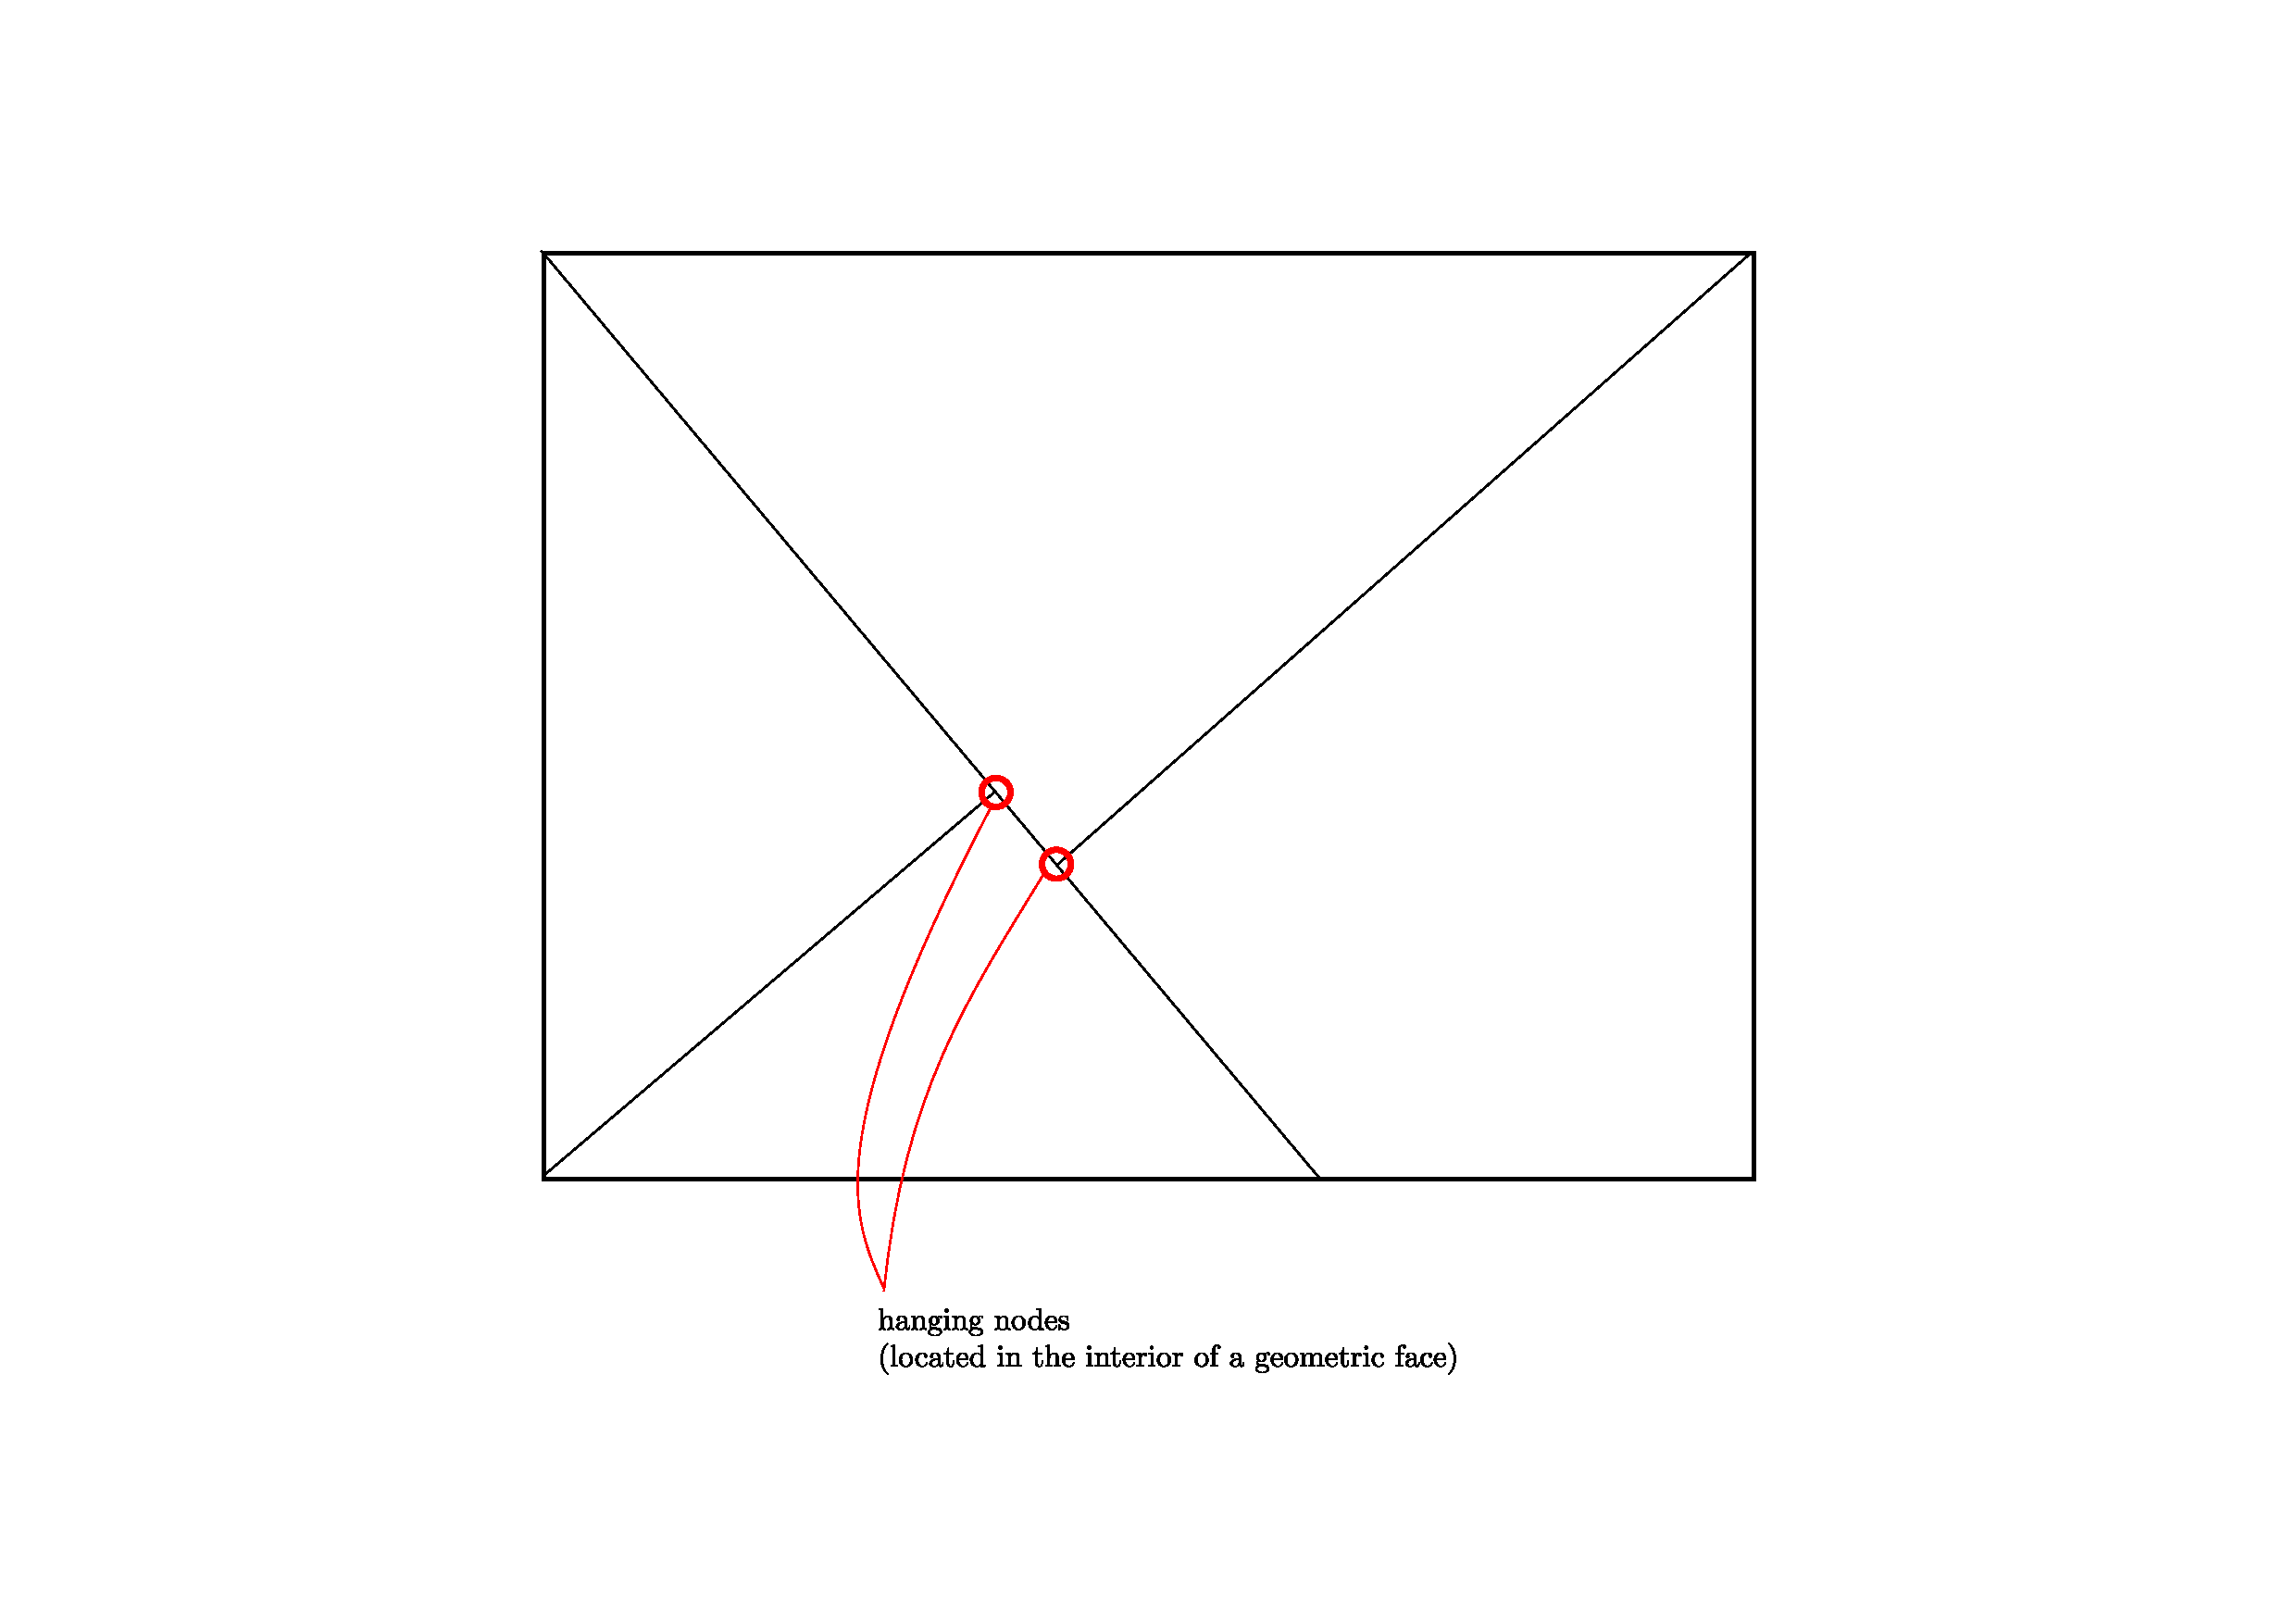
\includegraphics[width=\textwidth]{figs/hangingNodes.pdf}
      \end{center}
      \caption{hanging nodes}
      \label{hanging-nodes-figure}
    \end{figure}

  \item \emph{Grids} are meshes with translation invariant structure, these can be tensor product grids, that are meshes whose cells are quadrilaterals (d=2) or hexaedron (d=3)
    \begin{figure}[H]
      \begin{center}
        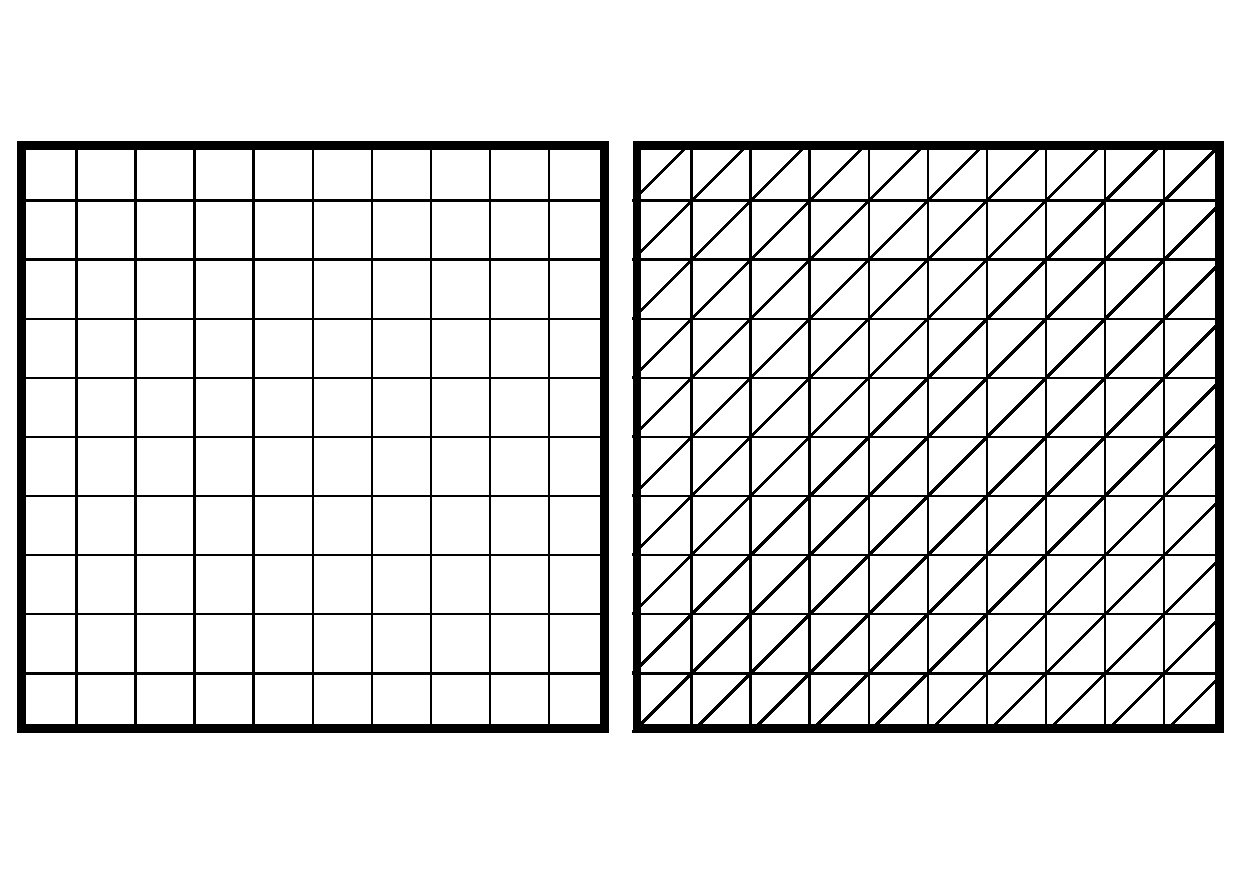
\includegraphics[width=\textwidth]{figs/grids.pdf}
      \end{center}
      \caption{different triangulations on grids}
      \label{grids-figure}
    \end{figure}
  \item the \emph{orientation} of a geometric objects of hte mesh is important when defining higher order basis functions.
    \begin{enumerate}
    \item for an edge we haev to define its directions
    \item for a face we have to specify an ordering of the edges along its boundary
      
    \end{enumerate}

  \end{itemize}
\end{defi}
\subsection{linear finite elements on triangular meshes}
Reference cell $\hat K \ (d=2)$
\begin{figure}[H]
  \begin{center}
    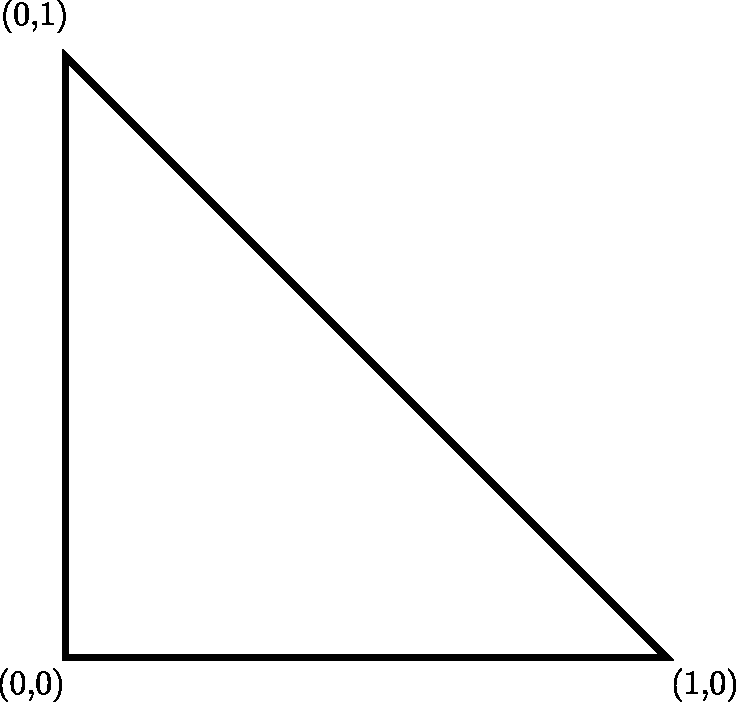
\includegraphics[width=\textwidth]{figs/referenceCell.pdf}
  \end{center}
  \caption{reference cell}
  \label{reference-cell-figure}
\end{figure}
\begin{itemize}
\item for triangles reference triangles with nodes (0,0),(1,0),(0,1)
\item quadrilaterals reference quad $[0,1]^2$ or $[-1,1]^2$
\end{itemize}
\begin{figure}[H]
  \begin{center}
    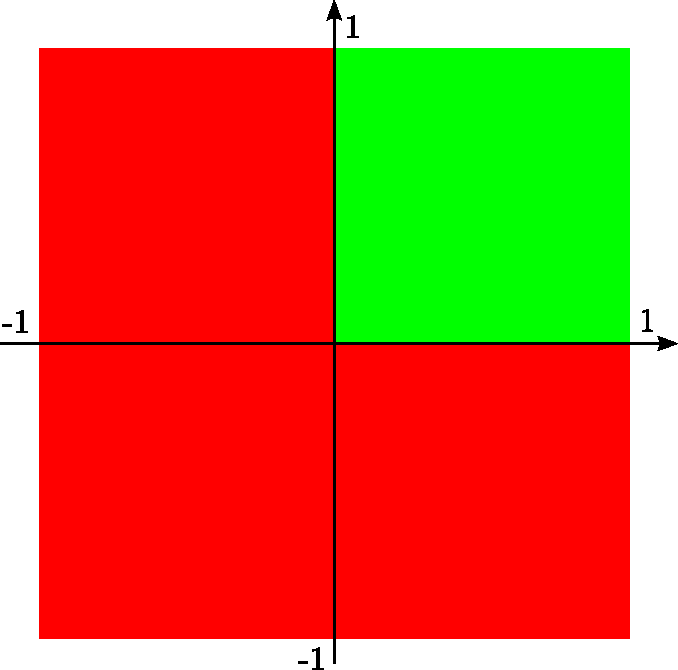
\includegraphics[width=\textwidth]{figs/quadrilaterals.pdf}
  \end{center}
  \caption{quadrilaterals}
  \label{quadrilaterals-figure}
\end{figure}

Affine mapping $\Phi$\\
linear bijective mapping from a refence cell(triangle or prarllelogramm) to a physical cell (triangle/parallelogramm) in the mesh $$\Phi : \RR^d \to \RR^d , \xi \to F \xi + \tau$$
$$F \in \RR^{d\times d} \tx{ is regular, } \tau \in \RR^d$$
A mesh is called \emph{affine equivalent} of all its cells arise as affine images of a single reference cell
\subsubsection{Basis functions}
$\OO\subset \RR^2$ is a lipschitz polygon\\
$\M$ is a conforming mesh of $\OO$ containing only triangles as cells.
\begin{defi} We define  the finite elements space of piecewise linear continous functions
  $$S^1 (\OO,\M) := \left\{u \in C^0 (\OO) : u(x)_{|K} = a+bx_1+cx_2 \ \forall K \in \M\right\}$$
\end{defi}
\begin{prop}
  \begin{itemize}
  \item $S^1 (\OO,\M) \subset H^1(\OO)$
  \item $u \in S^1(\OO,\M) $ is uniquely defined by the values u(P) on the nodes $P \in \N(\M)$
  \item N= dim$ S^1(\OO,\M) = |\N | <\infty$
  \item $S^1(\OO,\M) = span\ \left\{b_P(x) : P\in \N(\M) \right\} $ with so called functions $b_P \in S^1(\OO,\M) \ b_P(P') = \dd_{P=P'}, $ for all $P'\in \N(\M)$ ($\dd$ is the Kronecker symbol)
  \end{itemize}
\end{prop}
Let b be the vector of the basis function. Then an arbitary FE function $v \in  S^1(\OO,\M)$ can be written as 
$$v(x) = \sum_{P \in \N(\M)} v(P) b_P(x) = v^T b_P(x)$$
\subsubsection{Assembling system matix and load vector}
\begin{figure}[H]
  \begin{center}
    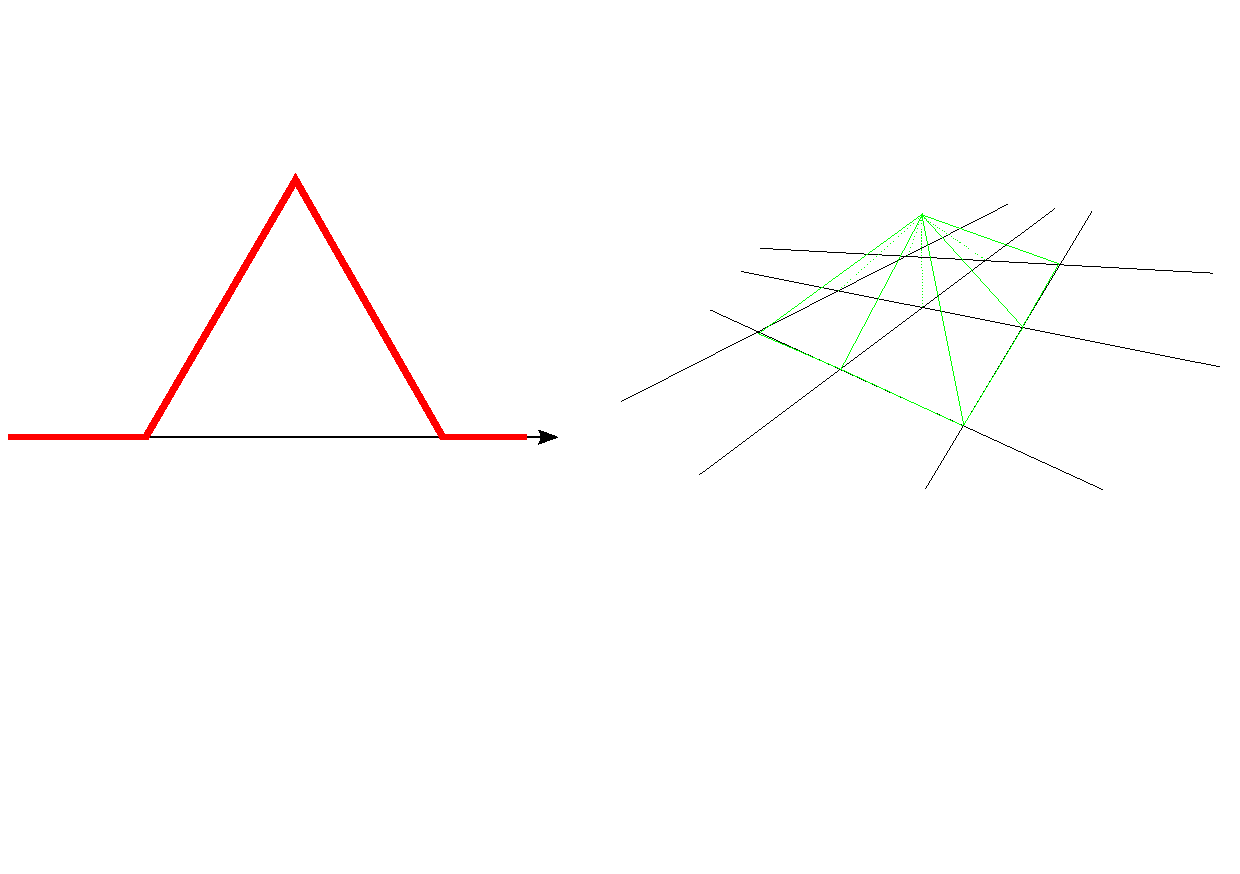
\includegraphics[width=\textwidth]{figs/hatFunction.pdf}
  \end{center}
  \caption{hat functions in 2d and 3d}
  \label{hat-functions-figure}
\end{figure}

Consider shape functions, that are restrictions of the basis functions to one cell $K \in M$ For $S^1(\OO,\M)$ these are exactly three, each for one nod of K. 
\begin{figure}[H]
  \begin{center}
    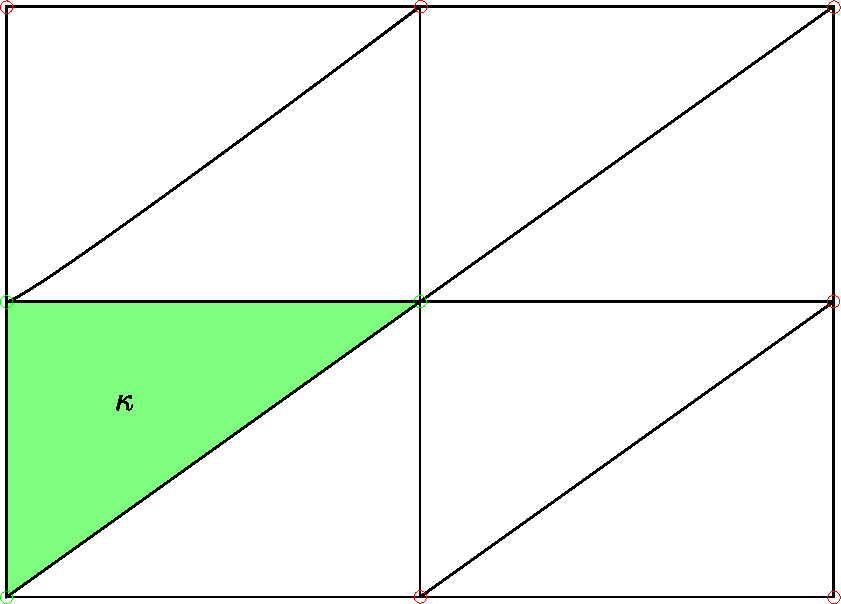
\includegraphics[width=\textwidth]{figs/shapeFunctions.pdf}
  \end{center}
  \caption{shape function}
  \label{shape-function-figure}
\end{figure}

The shape functions can be defined on a single cell K as 
$$N_{K,P_j(K)}(x) = \hat N_j(\Phi^{-1}_K x)$$
where the element shape functions are defined by $\hat N_0(\xi ) = 1 - \xi_1-\xi_2, \ \hat N_1(\xi) =\xi_1 , \ \hat N_2(\xi) = \xi_2  $ on the reference cell $\hat K$\\
\begin{figure}[H]
  \begin{center}
    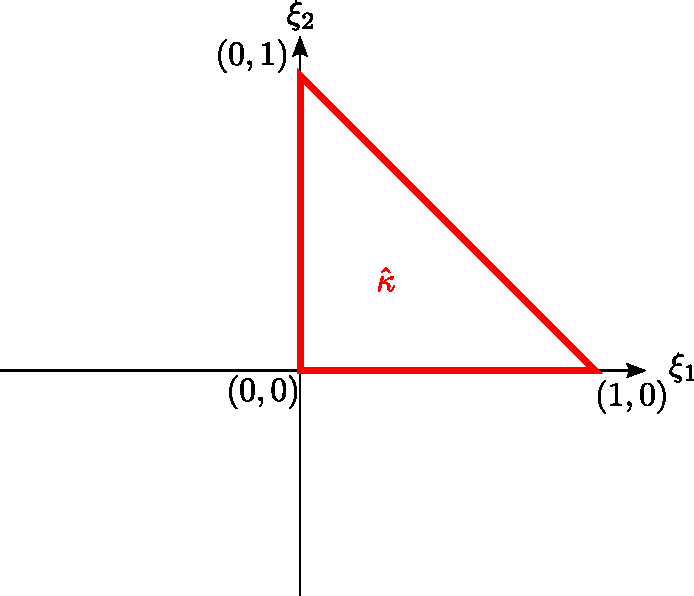
\includegraphics[width=\textwidth]{figs/referenceCellKappaHat.pdf}
  \end{center}
  \caption{reference cell}
  \label{ref-cell-kappa-hat-figure}
\end{figure}

$P_j(K) $ is the j-th node of the triangle K, j=0,1,2 with coordinates $p_j$. Then the (affine) element mapping reads 
$$x= \Phi_k(\xi) = p_0 + \xi(p_1-p_2)+\xi(p_2-p_0) = \tau + \F_k \xi$$
with $\F_k= (p_1-p_0,p_2-p_0) , \ \tau = p_0$
% \end{defi}
\printindex  % create the index at the end



missing lecture 8.5.2014




\end{document}

